\problemname{Problem 6 - Summit}

Professor Plum likes vacationing in the mountains.  He wants you to consider this mathematical mountain, where each non-leaf node is the sum of its two children:

\begin{figure}[h]
\begin{center}
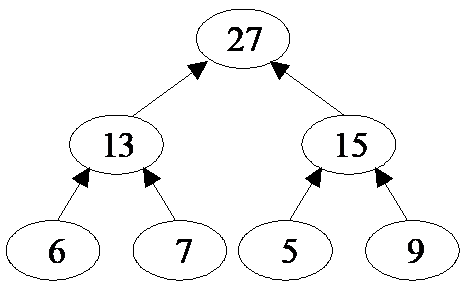
\includegraphics[width=0.6\textwidth]{problem6tree.png} 
\end{center}
\end{figure}

Something’s wrong, however. $27 \neq 13 + 15$, and 1$5 \neq 5 + 9$. If we replace the $15$ with $14$, then we have a well-formed mathematical mountain. Given a serialized version of a mountain, where the root is element $0$, the root’s left and right children are elements $1$ and $2$, and so on down the mountain, print the index of the single incorrect element and the corrected value.  If the incorrect value occurs on the leaf level, then the right child is assumed to be wrong.

\section*{Input}
The input consists of a number of cases followed by a line for each tree. The first number on a mountain’s line is the number of levels in the mountain. The remaining numbers are the node values, separated by whitespace and in breadth-first order. A mountain will always have at least $3$ levels. Each mountain is full and complete, meaning that all non-leaves have exactly two children and that all leaves are on the bottom-most level.

\section*{Output}
For each case, print a case label, the index of the incorrect node, and the correct value. For the example input, the output is: